% --------------------------------------------------------------------
% --------------------------------------------------------------------
% ---- DO NOT CHANGE THIS BLOCK OF CODE
\documentclass[abstract=true]{scrartcl}

\usepackage[fleqn]{amsmath}
\usepackage{amssymb}

\usepackage[T1]{fontenc}
\usepackage[margin=1in]{geometry}
\usepackage{fancyhdr}
\usepackage{graphicx}

% this is used for the dummy latin text 
\usepackage{lipsum}

% to typeset algorithms
\usepackage{algorithm}
\usepackage{algpseudocode}

% to typeset code blocks
\usepackage{minted}
\usepackage{xcolor}

% to manage URLs 
\usepackage{hyperref}
\hypersetup{
    colorlinks=true,
    linkcolor=blue,
    filecolor=magenta,      
    urlcolor=teal,
    pdftitle={Overleaf Example},
    pdfpagemode=FullScreen,
    citecolor=red,
}


% for bibliography management and reference list
\usepackage[sort&compress,numbers]{natbib}
\bibliographystyle{abbrvnat}

 
\pagestyle{fancy}
\fancyhf{}
\chead{Mini Project Report}
\lhead{DS3294: DS Practice}
\cfoot{\thepage}

% DO NOT change the subtitle
\subtitle{Mini Project for DS3294: Data Science Practice}
\date{\small \today}
% --------------------------------------------------------------------
% --------------------------------------------------------------------

% --------------------------------------------------------------------
% --------------------------------------------------------------------
% ---- ENTER YOUR PROJECT DETAILS BELOW

% ---- title of the project
\title{Demographic Data Dashboard for India}

% ---- names of team members
\author{
    \small Gaurav Chandan \and
    \small Soumya Ranjan \and
    \small Shweta Shankar \and
    \small Dheeraj Kumar Gehlot
    }

% ---- enter the team number below
\rhead{Team Number 03}

% --------------------------------------------------------------------
% --------------------------------------------------------------------


% --------------------------------------------------------------------
% --------------------------------------------------------------------
% ---- DO NOT CHANGE THIS BLOCK OF CODE
\begin{document}
\maketitle
% --------------------------------------------------------------------
% --------------------------------------------------------------------



% --------------------------------------------------------------------
% --------------------------------------------------------------------
% ---- WRITE YOUR REPORT BELOW

\section{Introduction}
India is currently undergoing a massive demographic transition, marked by falling fertility rates, rising life expectancy, and a historical peak in the working-age population share. Understanding these changes across various states and districts is crucial for policy making and socio-economic planning. This project aims to build an end-to-end data pipeline to ingest, clean, analyze, and visualize demographic data for India. The interactive dashboard developed facilitates the exploration of regional disparities and relationships between key indicators spanning population dynamics, economics, healthcare, literacy, and urbanization.
\\\\
\href{https://indiametrics.streamlit.app}{Click here to view the dashboard.}

\section{Related Work}
Demographic studies of India have long relied on decadal Census data and sample surveys. Previous efforts typically provided static reports or siloed dashboards focusing only on either healthcare (e.g., NFHS reports) or economic proxies. Interactive tools combining data from the Census, World Bank, VAHAN, and District Level Household Surveys directly to explore the demographic-economic transition are relatively uncommon. This project bridges that gap by offering a unified dashboard combining multiple data sources to better understand regional demographic shifts.

\section{Our contribution}
Our contributions include:
\begin{itemize}
    \item Integration of multiple datasets (Census 2001/2011, World Bank, data.gov, VAHAN EV/CNG registries).
    % \item Development of a standardized data clearing pipeline to resolve state/district naming inconsistencies and temporal granularity differences.
    \item Creation of a scalable and interactive Streamlit dashboard mapping state and district level trends from 1971 to 2011 and beyond.
    \item Computation of a Composite Demographic Health Index to summarize the overall well-being across Indian districts.
\end{itemize}

\section{Methods}
\subsection{Data}
The datasets include Population (Census 2001, 2011), Economic indicators (NSDP GDP, per capita income from data.gov), Healthcare metrics (fertility, mortality from DLHS and SRS), and Literacy and Urbanization figures. 
\\
Data cleaning involved standardization of column names, handling of missing values, and normalization of categorical strings such as state and district identifiers. Absolute numbers were normalized into robust rates, converting figures like Total Gross Domestic Product (GDP) into per capita equivalents and calculating literacy rates and rural-urban performance gaps.

\subsection{Data Pipeline and Dashboard Architecture}
The core application code is developed in Python. Data manipulation depends heavily on \verb|pandas| and \verb|numpy| for aggregating, filtering, and joining various datasets. Geo-spatial visualization relies on \verb|geopandas| aligning statistical information to district polygons (GeoJSON). Dashboard interactivity is managed by \verb|streamlit|, enhanced by \verb|plotly| for rendering dynamic choropleths, scatter plots, time-series, and radar charts. 
\\\\
The main dashboard (\verb|dashboard_v3.py|) follows a modular architecture dividing analytics into:
\begin{itemize}
    \item National Demographic Overview
    \item State Comparisons
    \item District Explorer
    \item Insights \& Correlations
\end{itemize}

\section{Results}
\subsection{National and State Trends}
The integration pipeline highlights the stark divergence among Indian states regarding demographic variables. States like Kerala and Tamil Nadu exhibit low Total Fertility Rates (TFR) below the replacement level (2.1), corresponding with higher literacy and per-capita incomes. In contrast, states such as Bihar and UP showcase the opposite pattern with higher TFRs pointing to an earlier stage of the demographic transition.

\subsection{Dashboard Interactive Experience}
The tool developed offers rich interactive components. Notably, users can toggle between absolute counters and per capita metrics. Plotly graphs provide deep drill-down capabilities such as a time-series animation of Green Mobility (EVs and CNG vehicle usage) and state-level comparative radar charts contrasting literacy, sex ratio, urbanization, per-capita income, and TFR simultaneously.

\subsection{Composite Demographic Health Index}
We designed a relative performance index summarizing four normalized components: literacy rate, sex ratio, inverted TFR, and urbanization percentage. The choropleth visualization of this index points to explicit geographical bandings, establishing a strong sub-national spatial correlation for overall human development across the subcontinent.

\section{Conclusion and Outlook}
In conclusion, the Demographic Data Dashboard successfully integrates diverse national datasets into an accessible exploratory tool. The insights reaffirm the classical demographic-economic transition theory on an intra-national scale in India.
\\\\
The demographic-economic transition theory posits that societies move through a predictable sequence of stages as they develop economically. In the first stage, both birth rates and death rates are high, resulting in slow population growth. As public health and nutrition improve, the second stage sees death rates fall sharply while birth rates remain elevated, producing rapid population growth. In the third stage, rising education levels --- particularly female literacy --- greater urbanization, and improved access to family planning drive birth rates downward. Finally, in the fourth stage, both birth and death rates stabilize at low levels and population growth plateaus or even reverses. 
\\\\
Our dashboard captures this transition playing out simultaneously across Indian states at different speeds: states like Kerala and Tamil Nadu have reached the late stages with sub-replacement fertility (TFR below 2.1), high literacy, and elevated per-capita incomes, while states such as Bihar and Uttar Pradesh remain in the earlier stages with higher TFRs and lower literacy. The strong negative correlation between literacy and TFR, and the positive association between per-capita income and lower fertility observed in our analysis, provide direct empirical support for this theoretical framework at the sub-national level (see Appendix \ref{sec:dashboard_plots} for visual evidence). Specifically, Figure \ref{fig:tfr_mcpr} is useful for demonstrating the strong negative correlation between fertility rates and contraceptive prevalence, validating that access to family planning directly lowers TFR across states. Figure \ref{fig:life_expectancy} is useful to visualize the steady historical rise in life expectancy, confirming improved healthcare and nutrition as mortality falls in the second stage of the transition. Lastly, Figure \ref{fig:crude_rates} is useful as it beautifully captures the "vital transition" where the crude birth rate starts narrowing the gap with the crude death rate, proving that long-term population growth is beginning to stabilize.
\\\\
Future work will involve integrating newer census data (once available) and possibly applying predictive models to forecast state and district-level outcomes. 

\section{Acknowledgements}
We acknowledge data.gov.in \cite{datagov}, the World Bank \cite{worldbank}, and the Census of India \cite{census2011} for making their demographic datasets publicly available. We also utilized the VAHAN Dashboard \cite{vahan} for green mobility data.

\section{Author Contributions}
Gaurav Chandan, Soumya Ranjan, Shweta Shankar, and Dheeraj Kumar Gehlot contributed equally to data collection, pipeline engineering, dashboard development, and report writing.

\section{Code availability}
The \href{https://github.com/gauravchandan/DS-Practice-2026-Team-3}{project repository} containing all the source code is available on Github, and the interactive dashboard can be accessed on \href{https://indiametrics.streamlit.app}{Streamlit Community Cloud}.

% --------------------------------------------------------------------
% --------------------------------------------------------------------
% ---- DO NOT CHANGE THIS BLOCK OF CODE
\section{References}
\bibliography{refs}
% --------------------------------------------------------------------
% --------------------------------------------------------------------


\section{Appendix}



\subsection{Code snippets}

The snippet below shows how the dashboard cleans standard state names before data assimilation.

\begin{minted}[bgcolor=white, fontsize=\small, linenos, frame=none]{python}
def clean_state(s):
    if not isinstance(s, str): return s
    s = s.strip().title().replace('&', 'And')
    s = s.replace('Nct Of Delhi', 'Delhi').replace('The Nct Of Delhi', 'Delhi')
    s = s.replace('Islands', '').strip()
    return s
\end{minted}

The snippet below shows how the choropleth maps are generated for the spatial visualization of district-level metrics using \verb|px| (the commonly used alias for \verb|plotly.express|, which provides a high-level API for rapid chart generation).

\begin{minted}[bgcolor=white, fontsize=\small, linenos, frame=none]{python}
def build_choropleth(df_target, location_col, color_col, title, hover_data=None, theme_scale=None):
    fig = px.choropleth_mapbox(
        df_target, geojson=geojson, featureidkey='properties.pc11_d_id',
        locations=location_col, color=color_col,
        color_continuous_scale=theme_scale, 
        hover_name='District_Name' if 'District_Name' in df_target.columns else 'State',
        hover_data=hover_data,
        mapbox_style="carto-darkmatter", center={"lat": 22, "lon": 83}, zoom=3.3
    )
    if 'geometry' in india_boundary.columns:
        fig.add_trace(get_boundary_trace(india_boundary))
    fig.update_layout(
        margin={"r":0,"t":40,"l":0,"b":0}, height=500, 
        paper_bgcolor=PAPER_BG, plot_bgcolor=PLOT_BG,
        title=title, title_font=dict(color="#e5e5e5")
    )
    return fig
\end{minted}


The snippet below illustrates the World Bank data wrangling pipeline. Raw CSV data arrives in wide format with indicator series as rows and year columns containing mixed types and missing values denoted by \verb|'..'|. The pipeline melts it into long format, extracts numeric years via regex, coerces values, interpolates gaps within each series using bidirectional filling, and pivots back into a clean wide table indexed by year.

\begin{minted}[bgcolor=white, fontsize=\small, linenos, frame=none]{python}
df_wb = pd.read_csv(os.path.join(DATA_DIR, "WorldBank_Final.csv")).replace('..', np.nan)
df_wb_melt = df_wb.melt(id_vars=['Series Name'], var_name='YearRaw', value_name='Value')
df_wb_melt['Year'] = df_wb_melt['YearRaw'].str.extract(r'(\d{4})').astype(float)
df_wb_melt['Value'] = pd.to_numeric(df_wb_melt['Value'], errors='coerce')
df_wb_melt['Value'] = df_wb_melt.groupby('Series Name')['Value'].transform(
    lambda x: x.interpolate(limit_direction='both')
)
df_wb_wide = df_wb_melt.dropna(subset=['Year']).pivot(
    index='Year', columns='Series Name', values='Value'
).reset_index()
\end{minted}

The following snippet computes the Composite Demographic Health Index. Each of the four component indicators (literacy rate, sex ratio, inverted TFR, and urbanization percentage) is min-max normalized to the 0--1 range across all states. The four scores are then averaged and scaled to 0--100 to produce a single summary index per state.

\begin{minted}[bgcolor=white, fontsize=\small, linenos, frame=none]{python}
def norm(s): 
    return (s - s.min()) / (s.max() - s.min())

merged_heat['Lit_score'] = norm(merged_heat['Literacy_Rate'])
merged_heat['SR_score']  = norm(merged_heat['Sex_Ratio'])
merged_heat['TFR_score'] = 1 - norm(merged_heat['TFR_2011'])  # Inverted: lower is better
merged_heat['Urb_score'] = norm(merged_heat['Urban_Pct'])
merged_heat['Composite_Index'] = (
    merged_heat['Lit_score'] + merged_heat['SR_score'] 
    + merged_heat['TFR_score'] + merged_heat['Urb_score']
) / 4 * 100
\end{minted}

The final snippet shows the Green Mobility aggregation from the VAHAN vehicle registry. It filters EV and CNG registrations, groups them by state and year, computes each state's green vehicle market share as a percentage of total registrations, and merges urbanization data for the animated scatter plot.

\begin{minted}[bgcolor=white, fontsize=\small, linenos, frame=none]{python}
is_green = df_vahan_state['fuel_type'].str.upper().str.contains('CNG|ELECTRIC', na=False)
cg_ev = df_vahan_state[is_green].groupby(
    ['state_name', 'year']
)['registrations'].sum().reset_index()

tot = df_vahan_state.groupby(
    ['state_name', 'year']
)['registrations'].sum().reset_index()
tot.rename(columns={'registrations': 'tot_reg'}, inplace=True)

v_merge = pd.merge(cg_ev, tot, on=['state_name', 'year'])
v_merge['Green_Pct'] = (v_merge['registrations'] / v_merge['tot_reg']) * 100
\end{minted}

\subsection{AI Usage Declaration}
Large language models were employed in the development process to iterate on manual work done by the authors improve presentability and add visual appeal to the dashboard. The datasets were collected and cleaned manually from the sources listed above. Underlying ideas and the resulting insights are largely due to the authors.
\\\\
The datasets and authored code passed as prompts to the AI can be found in the \verb|Preliminary_Work| folder and the non-main branches of the Github repository.

\subsection{Useful Plots}
\label{sec:dashboard_plots}

\begin{figure}[htbp]
    \centering
    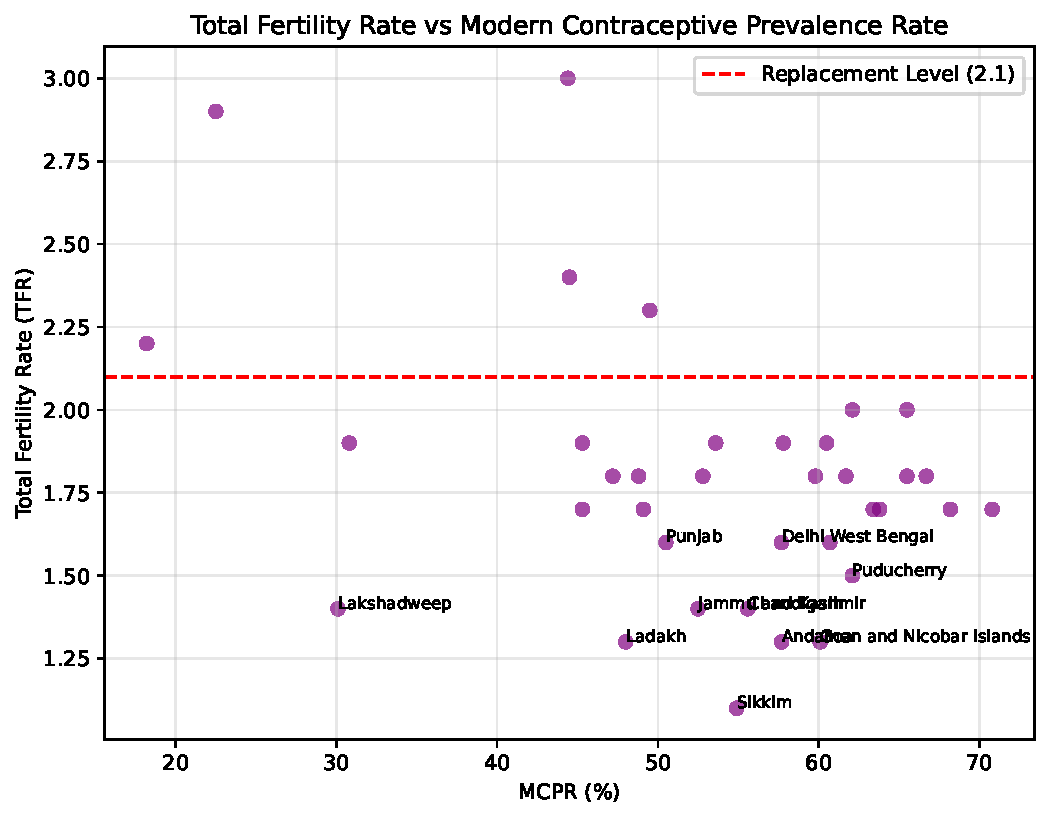
\includegraphics[width=0.8\textwidth]{figs/tfr_vs_mcpr.pdf}
    \caption{Total Fertility Rate vs Modern Contraceptive Prevalence Rate highlighting the strong negative correlation and demographic divergence across Indian states.}
    \label{fig:tfr_mcpr}
\end{figure}
\begin{figure}[htbp]
    \centering
    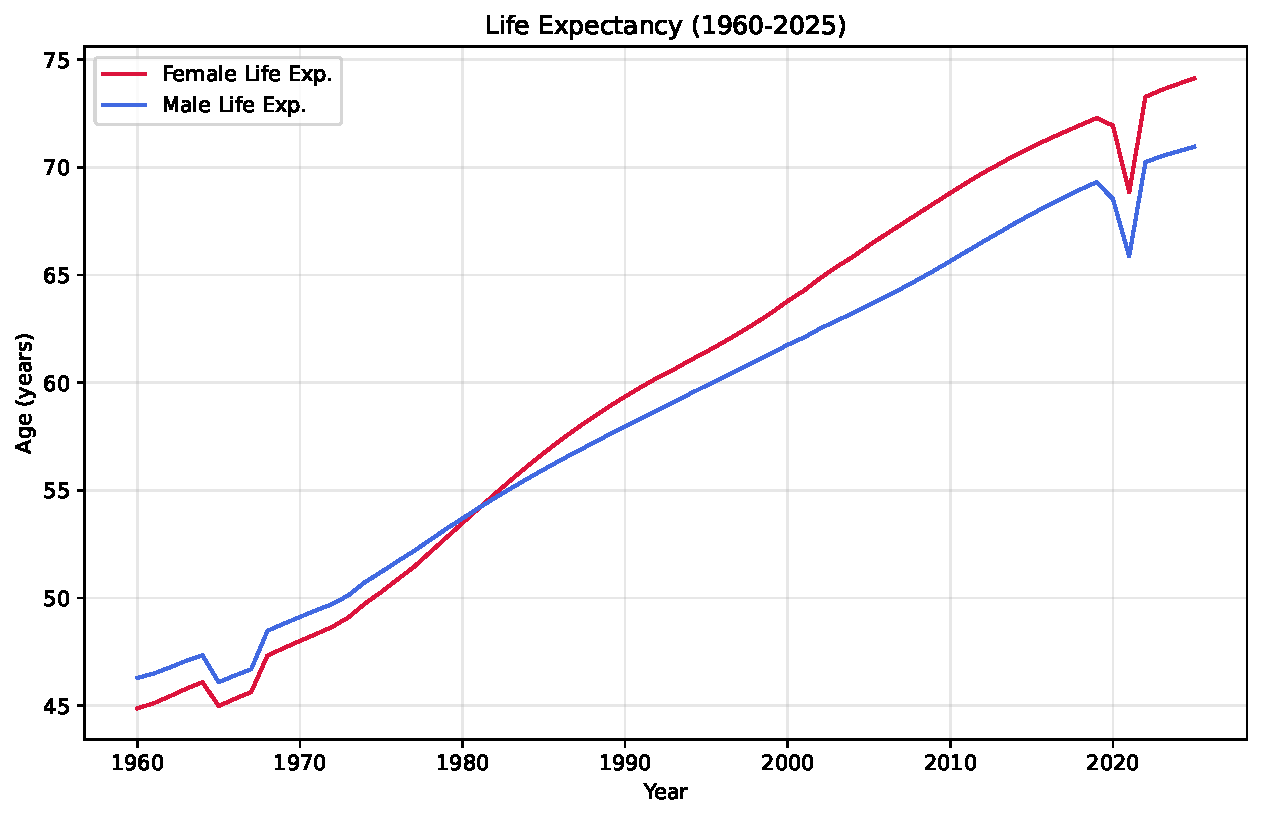
\includegraphics[width=0.8\textwidth]{figs/life_expectancy.pdf}
    \caption{Life expectancy trends in India (1960–2025). The graph demonstrates the success of long-term public health improvements that characterize the second stage of the demographic transition.}
    \label{fig:life_expectancy}
\end{figure}
\begin{figure}[htbp]
    \centering
    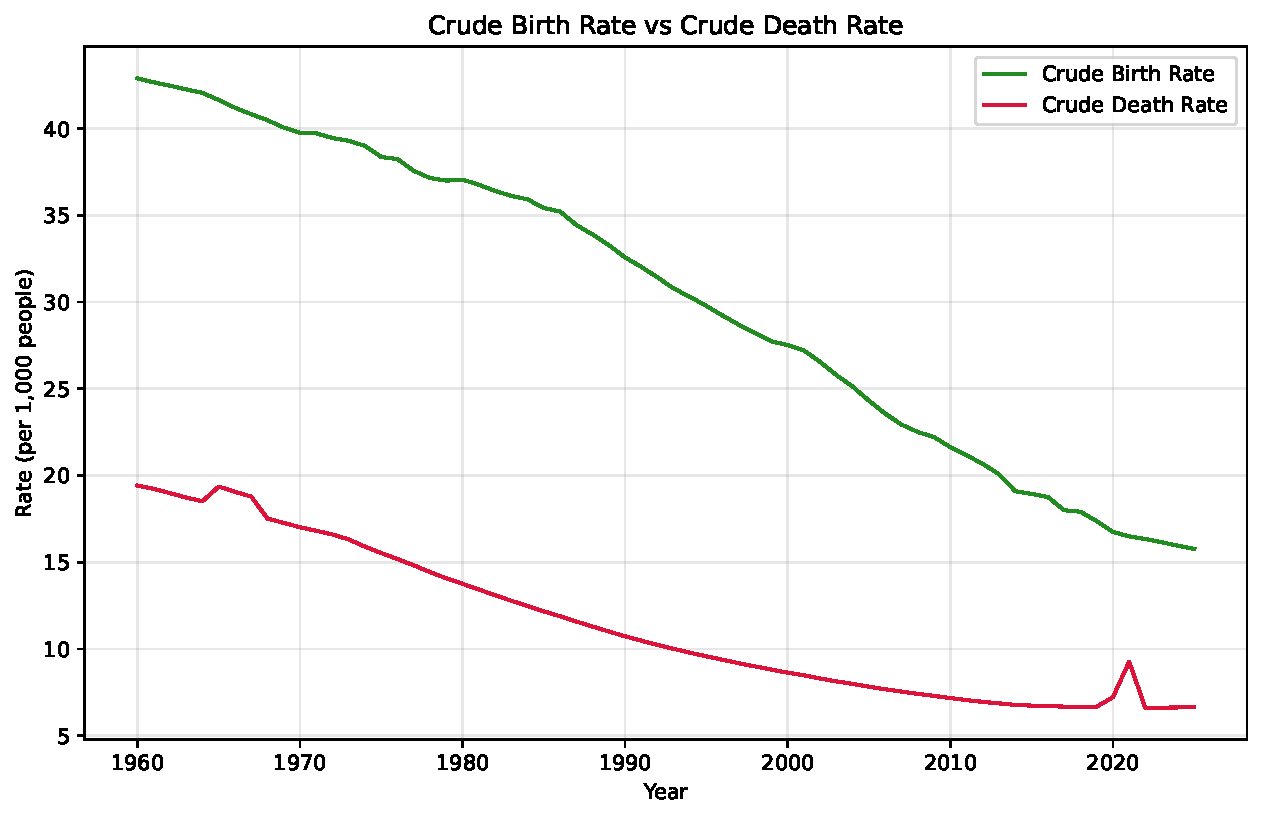
\includegraphics[width=0.8\textwidth]{figs/crude_rates.pdf}
    \caption{Crude Birth Rate vs Crude Death Rate in India (1960-2025). The crossing of these rates visually captures the 'vital transition', a core component of the demographic-economic transition theory.}
    \label{fig:crude_rates}
\end{figure}

% --------------------------------------------------------------------
% --------------------------------------------------------------------
% ---- DO NOT CHANGE THIS BLOCK OF CODE
\end{document}
% --------------------------------------------------------------------
% --------------------------------------------------------------------
